\subsection{Statistics for Measurement Data}
	\subsubsection{Q-Q Plot}
		\RTheory
		{					
			1. For
			\begin{center}
				$\alpha_k=\frac{k-0.5}{n}$ with $k=1,...,n$\\
			\end{center}
			
			calculate the corresponding theoretical quantiles of the model distribution
			
			\begin{center}
				$q(\alpha_k)=F^{-1}(\alpha_k)$\\
			\end{center}				 
			
			2. Determine the empirical $\alpha_k$-quantiles,
			
			\begin{center}
				$x_{(1)}<x_{(2)}<...<x_{(n)}$\\
			\end{center}				 
			
			3. Plot the empirical quantiles $x_k$ on the y-axis against the theoretical quantiles 					$q(\alpha_k)$ on the x-axis.		 
		}
		{
			sections/ProbabilityStatistics/StatisticsForMeasurementData/RCode/QQPlot.R
		}
		
		\begin{figure}[H]
			\begin{minipage}[c]{0.5\textwidth}
				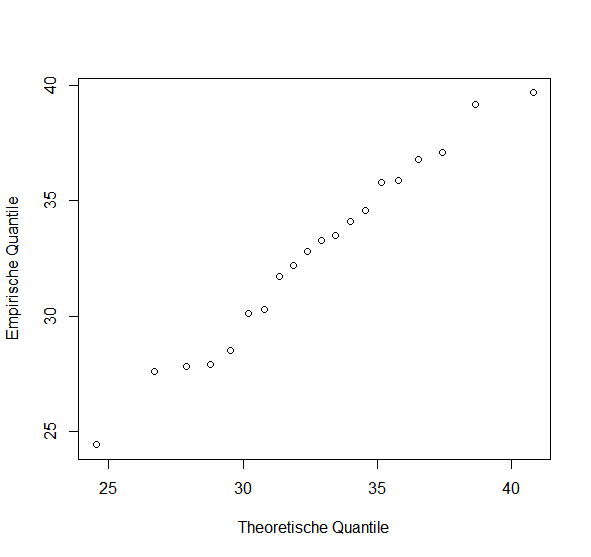
\includegraphics[width=1\linewidth]{images/qqPlot.png}
			\end{minipage}\hfill
			\begin{minipage}[c]{0.5\textwidth}
				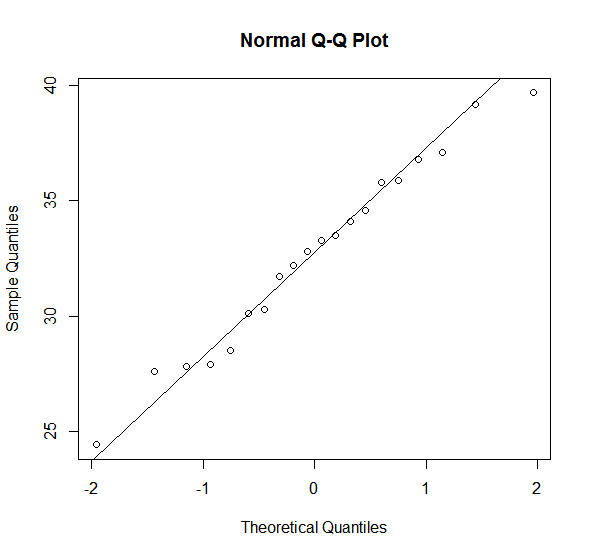
\includegraphics[width=1\linewidth]{images/qqNormLine.png}
			\end{minipage}\\
			\begin{minipage}[t]{.5\textwidth}
				\subcaption{qqplot()}
			\end{minipage}\hfill
			\begin{minipage}[t]{.5\textwidth}
				\subcaption{qqnorm();qqline()}
			\end{minipage}
		\end{figure}
		\begin{figure}[H]
			\begin{minipage}[c]{0.5\textwidth}
				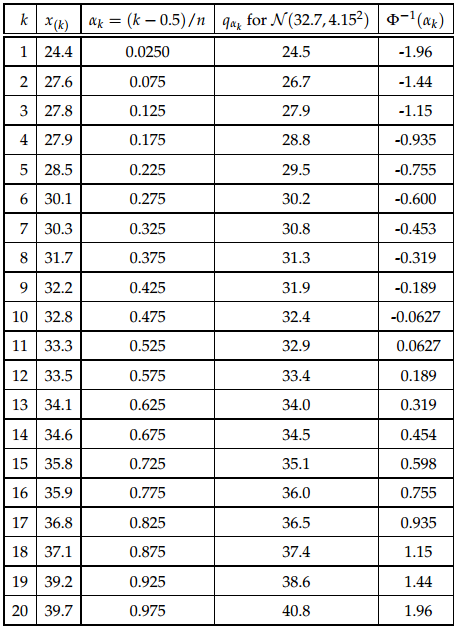
\includegraphics[width=1\linewidth]{images/qqList.png}
			\end{minipage}
			\begin{minipage}[c]{0.5\textwidth}
				\lstinputlisting[style=R]{sections/ProbabilityStatistics/StatisticsForMeasurementData/RCode/QQList.R}
			\end{minipage}
		\end{figure}

	\subsubsection{Parameter Esitmation for Continuous Probability Distributions}
	{
		% Extra row height for fractions and integrals
		\setlength{\extrarowheight}{3pt}
	
		\begin{twoColTable}
			\hline
			\twoColHdrRow{Method of Moments (not unbiased)}\\
			\hline
			\endhead
			Random variables							
				& $X_1,X_2,...,X_n$ \\
			\hline
			Measurements of these random variables (realisations, originating from same distribution)		
				& $x_1,x_2,...,x_n$ \\
			\hline
			Expected value
				& $\mu = E(X)  \Rightarrow \hat{\mu}=\bar{x}_n=\frac{x_1+x_2+...+x_n}{n}$\\
			\hline
			Variance
				& $\sigma^2 = E(X^2)-E(X)^2 = E(X^2)-\mu^2$\\
				& $\hat{\mu}^2+\hat{\sigma}^2 = \frac{1}{n}\sum\limits_{i=1}\limits^n x_i^2$\\
				& $\hat{\sigma}^2 = \frac{\sum\limits_{i=1}\limits^n(x_i-\bar{x}_n)^2}{n}$\\
				& $\hat{\sigma}^2 = \sqrt{\frac{1}{n}\sum\limits_{i=1}\limits^n(x_i-\hat{\mu})^2}$\\
			\hline
		\end{twoColTable}
		
		
		\begin{twoColTable}
			\hline
			\twoColHdrRow{Method of Maximum Likelihood}\\
			\hline
			General idea
				& Estimate a generic parameter (named $\theta$, which may represent $\mu$, $\lambda$\ldots) in such a way that the likelihood is maximized, that is, that it makes the observed data most likely or most probable.\\
			\hline
			$n$ observations of random variables, that are i.i.d.
				& $X_1=x_1,X_2=x_2,...,X_n=x_n$\\
			\hline
			\twoColHdrRow{Discrete probability distribution:}\\
			\hline
			Probability that random variable $X_i$ takes the value $x_i$
				& $P[X_i=x_i]$\\
			\hline
			Probability that the observations actually occurred
				& 
					{$\begin{aligned}
						&P[(X_1=x_1)\cap (X_2=x_2)\cap ... \cap (X_n=x_n)]\\
						&= P[X_1=x_1]\cdot P[X_2=x_2]\cdot ... \cdot P[X_n=x_n]\\
						&= \prod\limits_{i=1}\limits^n P[X_i = x_i]
					\end{aligned}$}\\
			\hline
			Generic probability distribution parameter (e.g. $\mu$, $\lambda$\ldots)
				& $\theta$\\
			\hline
			Likelihood function:\newline Probability that the $n$ measurements of independent random variables are observed.
				& 
					{$\begin{aligned}
						&L(\theta) = P[X_1=x_1|\theta]\cdot P[X_2=x_2|\theta]\cdot ... \cdot P[X_n=x_n|\theta]\\
						&= \prod\limits_{i=1}\limits^n P[X_i = x_i|\theta]
					\end{aligned}$}\\
			\hline
			Probability that random variable $X_i$ takes the value $x_i$, given parameter $\theta$
				& $P[X_i = x_i|\theta]$\\
			\hline
			\twoColHdrRow{Continuous probability distributions :}\\
			\hline
			Probability density function 
				& $f(x;\theta)$.\\
			\hline 
			Probability that each observation $x_i$ falls into its corresponding interval $[x_i , x_i + dx_i]$
				& $\prod\limits_{i=1}\limits^n f(x_i; \theta)dx_i$\\
			\hline
			Infinitesimal intervals $dx_i$ do not depend on the parameter value $\theta$, we omit them in the likelihood function
				& $\prod\limits_{i=1}\limits^n f(x_i; \theta)$\\
			\hline
			\twoColHdrRow{Example: Maximum Likelihood for Exponential Distribution}\\
			\hline
			Random variables
				& $X_1, X_2 . . . , X_n$ i.i.d. $\sim$ Exp($\lambda$)\\
			\hline
			Probability density function 
				& $f(x_i; \lambda) = \lambda e^{-\lambda x_i}$\\
			\hline
			Likelihood function for a given data set
				& $L(\lambda) = \prod\limits_{i=1}\limits^n \lambda e^{-\lambda x_i}$\\
			\hline
			Log likelihood function
				& $\log(L(\lambda)) = n \log(\lambda) - \lambda \sum\limits_{i=1}\limits^n x_i$\\
			\hline
			Derivative of the log likelihood function with respect to $\lambda$ and set it to $0$
				& $\frac{d \log(L(\lambda))}{d\lambda}=\frac{n}{\lambda}-\sum\limits_{i=1}\limits^n x_i \overset{!}{=} 0$\\
			\hline
			Maximum likelihood estimate
				& $\hat\lambda = \frac{n}{\sum\limits_{i=1}\limits^n x_i}=\frac{1}{\bar{x}}$\\
			\hline	
		\end{twoColTable}
	}

	\subsubsection{Statistical Tests and Confidence Interval for Normally Distributed Data}
	{
		% Extra row height for fractions and integrals
		\setlength{\extrarowheight}{3pt}
				
		\begin{twoColTable}
			\hline
			\twoColHdrRow{$z$-Test ($\sigma_x$ known)}\\
			\hline
					1. Model:
					& $X_1,...,X_n$ i.i.d. $\sim N(\mu, \sigma_{X}^2)$, $\sigma_X$ known\\
			\hline	
					2. Null hypothesis:
					& $H_0$:	$\mu=\mu_0$\\
					Alternative:
					& $H_A$:	$\mu \neq \mu_0$	(or $<$ or $>$)\\
			\hline	
					3. Test statistic:
					& $Z=\frac{(\bar{X}_n - \mu_0)}{\sigma_{\bar{X}_n}}=\frac{(\bar{X}_n - \mu_0)}{\sigma_{X_n}/\sqrt{n}}=\frac{\sqrt{n}(\bar{X}_n - \mu_0)}{\sigma_{X_n}}=\frac{observed-expected}{standard\,error}$\\
					Null distribution (assuming $H_0$ is true):
					&$Z \sim N(0,1)$\\
			\hline
					4. Significance level:
					& $\alpha$\\
			\hline
					5. Rejection region for the test statistic:
					& $K=(-\infty,z_{\frac{\alpha}{2}}] \cup [z_{1-\frac{\alpha}{2}}, \infty)$ with $H_A: \mu \neq \mu_0$, \vfill 
					$K=(-\infty,z_\alpha]$ with $H_A: \mu < \mu_0$, \vfill
					$K=[z_{1-\alpha}, \infty)$ with $H_A: \mu > \mu_0$\\
					where
					& $z_{\frac{\alpha}{2}} = \Phi^{-1}(\alpha/2)$\\
			\hline
					6. Test decision:
					& Check whether the observed value of the test statistic falls into the rejection region.\\
			\hline
		\end{twoColTable}
	
		\begin{figure}[H]
		    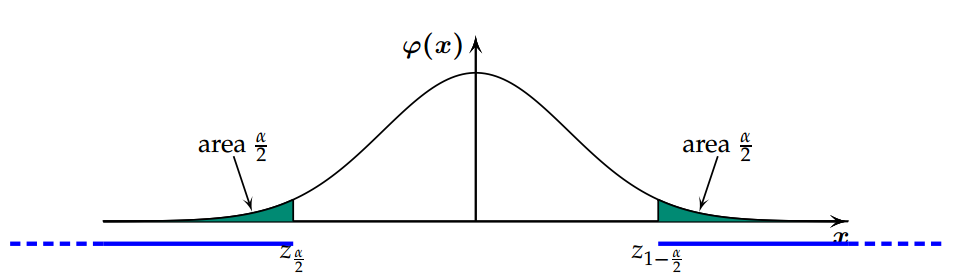
\includegraphics[width=1\linewidth]{images/zTestDecision.png}
		    \caption{z-Test: Rejection Region}
		\end{figure}
		
		\begin{twoColTable}
			\hline
			\twoColHdrRow{$z$-Test ($\sigma_x$ known): Standardized example}\\
			\hline
			Measurement of fusion heat:
				& The empirical mean value of $n=13$ measurements is $80.02$. From previous measurements the standard deviation is $\sigma_X = 0.01$. Is a fusion heat of exactly $80.00\frac{g}{cal}$ plausible?\\
			\hline
			Model:
				& $X_1,...,X_n$ i.i.d. $\sim N(\mu, \sigma_{X}^2)$, $\sigma_X=0.01$ known, $n=13$\\
			\hline	
			Null hypothesis:
				& $H_0$:	$\mu=\mu_0=80.00$\\
			Alternative:
				& $H_A$:	$\mu \neq \mu_0$\\
			\hline	
			Test statistic:
				& $Z=\frac{\sqrt{n}(\bar{X}_n - \mu_0)}{\sigma_{X_n}}$\\
			\hline
			Null distribution (assuming $H_0$ is true):
				&$Z \sim N(0,1)$\\
			\hline
			Significance level:
				& $\alpha = 0.05$ (commonly used $\alpha$-level)\\
			\hline
			Given $\alpha = 0.05$, {\color{blue}R} yields the following 2.5$\%$ quantile of the standard normal distribution.
				& {\lstinputlisting[style=R]{sections/ProbabilityStatistics/StatisticsForMeasurementData/RCode/zTest.R}}\\
			Rejection region for the test statistic (with the quantile returned from {\color{blue}R}):
				& 
					 {$\begin{aligned}
						z_{\frac{\alpha}{2}} &= \Phi^{-1}(\alpha/2) = \Phi^{-1}(0.025)=-1.96\\
						K &= (-\infty,z_{\frac{\alpha}{2}}] \cup [z_{1-\frac{\alpha}{2}}, \infty) \quad \mathrm{with} \quad H_A: \mu \neq \mu_0\\
						K &= (-\infty,-1.96] \cup [1.96, \infty)
					 \end{aligned}$}\\
			\hline
			Test decision:
				& $z=\frac{\sqrt{n}(\bar{X}_n - \mu_0)}{\sigma_{X_n}}=\frac{\sqrt{13}(80.02 - 80.00)}{0.01}=7.211$\\
				& Therefore the observed value falls into the rejection region.\\
			\hline
		\end{twoColTable}
			
		\begin{twoColTable}
			\hline
			\twoColHdrRow{$z$-Test ($\sigma_x$ known): Not standardized example}\\
			\hline
			Measurement of fusion heat:
				& The empirical mean value of $n=13$ measurements is $80.02$. From previous measurements the standard deviation is $\sigma_X = 0.01$. Is a fusion heat of exactly $80.00\frac{g}{cal}$ plausible?\\
			\hline
			Model:
				& $X_1,...,X_n$ i.i.d. $\sim N(\mu, \sigma_{X}^2)$, $\sigma_X=0.01$ known, $n=13$\\
			\hline	
			Null hypothesis:
				& $H_0$:	$\mu=\mu_0=80.00$\\
			Alternative:
				& $H_A$:	$\mu \neq \mu_0$\\
			\hline
			Test statistic: (not standardized) 
				&$T$: $\bar{X}_n$\\
			\hline
			Null distribution (assuming $H_0$ is true):
				&$T\sim N(\mu_0,\frac{\sigma_{X}^{2}}{n}) = N(80,\frac{0.01^2}{13})$\\
			\hline
			Significance level:
				& $\alpha = 0.05$ (commonly used $\alpha$-level)\\
			\hline
			Given $\alpha = 0.05$, {\color{blue}R} yields the following 2.5$\%$ quantile of the standard normal distribution.
				&{\lstinputlisting[style=R]{sections/ProbabilityStatistics/StatisticsForMeasurementData/RCode/zTest2.R}}\\
			\hline
			Rejection region for the test statistic (with the quantile returned from {\color{blue}R}):
				& 
					{$\begin{aligned}
						K &= (-\infty,c_u] \cup [c_o, \infty) \quad \mathrm{with} \quad H_A: \mu \neq \mu_0\\
						K &= (-\infty,79.99] \cup [80.01, \infty)
					\end{aligned}$}\\
			\hline
		\end{twoColTable}
		
		\begin{twoColTable}
			\hline
			\twoColHdrRow{$t$-Test ($\sigma_x$ unknown)}\\
			\hline
			Model:
				& $X_1,...,X_n$ i.i.d. $\sim N(\mu, \sigma_{X}^2)$, $\sigma_X$ is estimated by $						\hat{\sigma}_X$\\
			\hline	
			Null hypothesis:
				& $H_0$:	$\mu=\mu_0$\\
			Alternative:
				& $H_A$:	$\mu \neq \mu_0$	(or $<$ or $>$)\\
			\hline	
			Test statistic:
				& $T=\frac{\sqrt{n}(\bar{X}_n - \mu_0)}{\hat{\sigma}_{X}}=\frac{observed-expected}						{estimated\,\,standard\,\,error}$\\
			\hline
			Null distribution (assuming $H_0$ is true):
				&$T \sim t_{n-1}$\\
			\hline
			Significance level:
				& $\alpha$\\
			\hline
			Rejection region for the test statistic:
				&  
					{$\begin{aligned}
						K &= (-\infty,t_{n-1;\frac{\alpha}{2}}] \cup [t_{n-1;1-\frac{\alpha}{2}}, \infty) \quad \mathrm{with} \quad H_A: \mu \neq \mu_0\\
						K &= (-\infty,t_{n-1;\alpha]} \quad \mathrm{with} \quad H_A: \mu < \mu_0\\
						K &= [t_{n-1;1-\alpha}, \infty) \quad \mathrm{with} \quad H_A: \mu > \mu_0
					\end{aligned}$}\\
			\hline
			Test decision:
				& Check whether the observed value of the test statistic falls into the rejection region.\\
		\hline
		\twoColHdrRow{Example}\\
			\hline
			Model:
				& $X_1,...,X_{13}$ i.i.d. $\sim N(\mu, \sigma_{X}^2)$, $\sigma_X$ is estimated, $\hat{\sigma}_X=0.024$\\
			\hline	
			Null hypothesis:
				& $H_0$:	$\mu=\mu_0=80.00$\\
			Alternative:
				& $H_A$:	$\mu \neq \mu_0$\\
			\hline	
			Test statistic:
				& $T=\frac{\sqrt{n}(\bar{X}_n - \mu_0)}{\hat{\sigma}_{X}}$\\
			\hline
			Null distribution (assuming $H_0$ is true):
				&$T \sim t_{n-1}$\\
			\hline
			Significance level:
				& $\alpha = 0.05$\\
			
			\hline
			$t$-value
				& $t_{12;1-\frac{\alpha}{2}}=t_{12;0.975}=2.179$\\
				&{\lstinputlisting[style=R]{sections/ProbabilityStatistics/StatisticsForMeasurementData/RCode/tTest.R}}\\
			\hline
			Rejection region for the test statistic:
				& 
					{$\begin{aligned}
						K &= (-\infty,t_{12;\frac{\alpha}{2}}] \cup [t_{12;1-\frac{\alpha}{2}}, \infty) \quad \mathrm{with} \quad H_A: \mu \neq \mu_0\\
						K &= (-\infty,-2.179] \cup [2.179, \infty)\\
					\end{aligned}$}\\
			\hline
			Test decision:
				&$\bar{x}=80.02$ and $\hat{\sigma}_X=0.024$\\
			Realized value of the test statistic
				&$t=\frac{\sqrt{n}(\bar{X}_n - \mu_0)}{\hat{\sigma}_{X}}=\frac{\sqrt{13}(80.02 - 80.00)}{0.024}=3.00$\\
				&The realized value falls into the rejection region. Therefore, the null hypothesis is rejected at 5$\%$ level.\\
			\hline
			\twoColHdrRow {Small {\color{blue}R} Example:}\\
			\hline
			Code
				& {\lstinputlisting[style=R]{sections/ProbabilityStatistics/StatisticsForMeasurementData/RCode/tTestRExample.R}}\\
			\hline
			Observed value of the test statistic:
				& $3.12$. \\
			Test statistic, \newline assuming null hypothesis is true:
				& $t$-distribution with $df = 12$ degrees of freedom.\\
			Observed mean value of the data:
				& $80.02$. \\
			\textbf{Confidence interval:}
				& Is the region of values for $\mu$, for which the corresponding statistical test does not reject the null hypothesis\\
			$95\%$ confidence interval \newline for the true mean
				& $[80.006, 80.035]$.\\
			{\color{blue}qt(p,df)}:
				& Calculates the quantile of the $t$-distribution based on the probability and the degrees of freedom\\
			{\color{blue}pt(q,df)}:
				& calculates the probabilty density based on the quantile and the degrees of freedom.\\
			\hline
		\end{twoColTable}
		
		\begin{twoColTable} 
			\hline
			\twoColHdrRow{$P$-Value}\\
			\hline
			Principle
				& Probability that the test statistic will take on a value that is at least as large as the observed value, provided the null hypothesis $H_0$ is true.
					\begin{itemize}
					    \item Reject $H_0 \quad \mathrm{if} \quad p-\mathrm{value} \leq \alpha$
					    \item Retain $H_0 \quad \mathrm{if} \quad p\mathrm{value} > \alpha$
					\end{itemize}\\
			\hline
			\twoColHdrRow{One-sided alternative hypothesis $H_A: \quad \mu > \mu_0$:}\\
			\hline
			Observed value of the statistics
				& $t=\frac{\sqrt{n}(\bar{X}_n - \mu_0)}{\hat{\sigma}_{X}}$\\
			\hline
			$p$-value
				& $p = P(T>t)$\\
			\hline
			\twoColHdrRow{Two-sided alternative hypothesis $H_A: \quad \mu \neq \mu_0$:}\\
			\hline
			Observed value of the test statistics
				& $t=\frac{\sqrt{n}|\bar{X}_n - \mu_0|}{\hat{\sigma}_{X}}$\\
			\hline
			$p$-value
			 	& $p = 2 \cdot P(T>|t|)$\\
			\hline
			\twoColHdrRow {Small {\color{blue}R} Example:}\\
			\hline
			One- and two-sided $p$-value
				& {\lstinputlisting[style=R]{sections/ProbabilityStatistics/StatisticsForMeasurementData/RCode/pValue.R}}\\
			\hline
		\end{twoColTable}
		
		\paragraph{Interpreting statistical test results of a Linear Model in R}
			\RExample
			{
				sections/ProbabilityStatistics/StatisticsForMeasurementData/RCode/ptTestsLMCode.R
			}
			{
				sections/ProbabilityStatistics/StatisticsForMeasurementData/RCode/ptTestsLMOutput.R
			}
			{
				\begin{tabular}{>{\bfseries}p{0.15\textwidth}p{0.75\textwidth}}
					t-value
						& Value of the test statistic, assuming null hypothesis is true: $t = \frac{\beta_i - \mu}{se(\beta_i)}= \frac{\beta_i - 0}{se(\beta_i)} = \frac{\mathrm{Estimate}}{\mathrm{Std. Error}}$\\
					Pr($>|t|$)
						& $p$-value. Probability of observing a value of the test statistic at least as large as the returned $t$-value. Reject the null hypothesis if this value is $<\alpha$\\
					R-squared\newline values
						& Values close to $1$: A large part of the variance of the data is explained by the model.\\
						& Values close to $0$: Little of the variance of the data is explained by the model.\\
					F-Statistic
						& Values close to $1$: There is no relationship between response and predictors.\\
						& Values greater than $1$: There is a relationship between response and predictors.\\
				\end{tabular}
			}
	}